\section{Results}
\label{sec:results}

\subsection{Deterministic private-data matrix}

\begin{table*}[t]
\centering
\caption{Person-level agreement with the triangulated pseudo-reference for the
verified deterministic experiment matrix. Values are in repository coordinate
units. The confidence interval is a fixed-seed percentile bootstrap over people
and does not establish absolute 3D accuracy. Lower MPJPE is better. The
pseudo-reference-fitted joint-weight row is a legacy diagnostic and is not an
eligible label-free comparator.}
\label{tab:deterministic-baselines}
\small
\resizebox{\linewidth}{!}{%
\begin{tabular}{r l r S[table-format=1.4] S[table-format=1.4] S[table-format=1.4] c c}
\toprule
Rank & Method & $N$ & {Mean} & {SD} & {Median} & {IQR} & {95\% CI of mean} \\
\midrule
1 & Sim3 + pseudo-reference-fitted joint weights (leaky diagnostic) & 137 & 0.0635 & 0.0160 & 0.0611 & [0.0521, 0.0706] & [0.0609, 0.0662] \\
2 & \textbf{Body-frame average (recommended leakage-free)} & 137 & 0.0640 & 0.0161 & 0.0623 & [0.0532, 0.0717] & [0.0615, 0.0668] \\
3 & Sim3 (stable joints) + average & 137 & 0.0646 & 0.0159 & 0.0616 & [0.0536, 0.0730] & [0.0621, 0.0673] \\
4 & Sim3 + body-part weights & 137 & 0.0649 & 0.0162 & 0.0621 & [0.0540, 0.0736] & [0.0622, 0.0676] \\
5 & Sim3 + side smoothing + average & 137 & 0.0655 & 0.0159 & 0.0628 & [0.0545, 0.0739] & [0.0629, 0.0682] \\
6 & Sim3 + average + output smoothing & 137 & 0.0663 & 0.0159 & 0.0640 & [0.0556, 0.0746] & [0.0637, 0.0690] \\
7 & Sim3 (all joints) + average & 137 & 0.0738 & 0.0195 & 0.0725 & [0.0601, 0.0828] & [0.0707, 0.0771] \\
8 & World-coordinate average & 137 & 0.1221 & 0.0184 & 0.1210 & [0.1082, 0.1325] & [0.1190, 0.1252] \\
9 & Root alignment + average & 137 & 0.1222 & 0.0184 & 0.1210 & [0.1082, 0.1326] & [0.1191, 0.1252] \\
\bottomrule
\end{tabular}
}
\end{table*}


The regenerated matrix contains one finite person-level result for each of nine
methods and 137 people (1,233 rows). The numerically smallest mean
pseudo-reference distance, 0.0635 repository units, belongs to the
pseudo-reference-fitted joint-weight diagnostic and is excluded from eligible
comparisons. Body-frame averaging is the lowest leakage-free method at 0.0640.
Relative to world-coordinate averaging (0.1221), canonical body-frame averaging
reduces the mean by 47.54\%. Stable-joint Sim3 averaging is close at 0.0646,
whereas all-joint Sim3 is 0.0738.

\begin{figure}
\centering
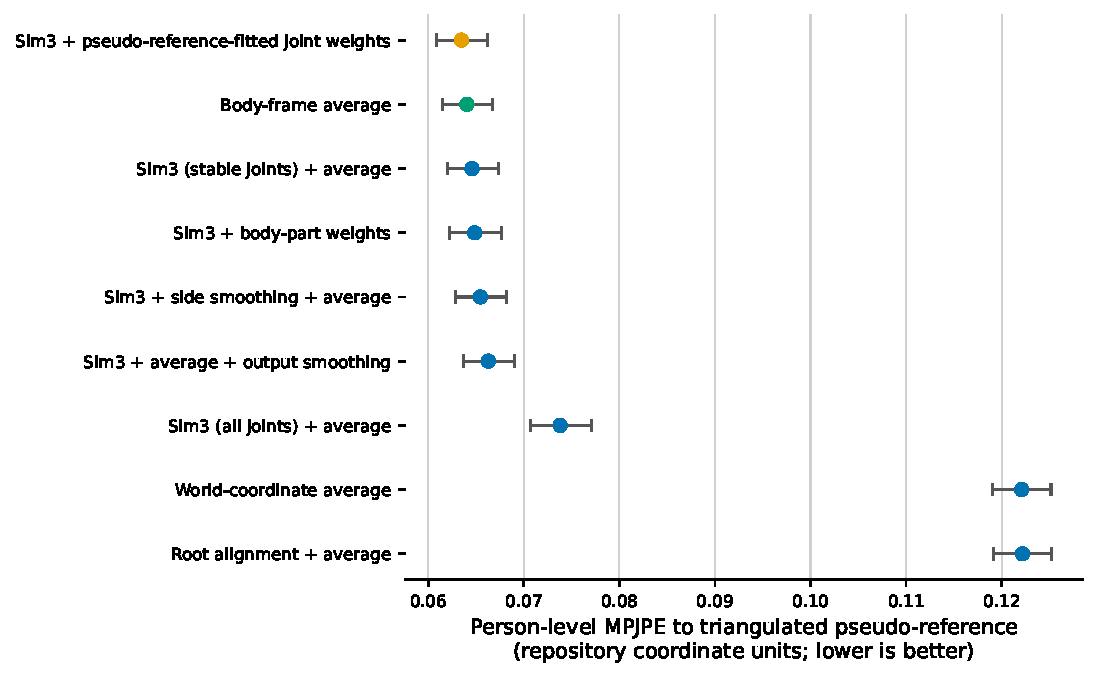
\includegraphics[width=\linewidth]{figures/deterministic_mpjpe.pdf}
\caption{Mean person-level distance to the same-video triangulated
pseudo-reference and fixed-seed 95\% bootstrap confidence interval for the
deterministic matrix. Units are repository coordinate units.}
\label{fig:deterministic}
\end{figure}

The strongest leakage-free intervals overlap. Accordingly, the deterministic
evidence supports canonicalization as the dominant operation, but does not
establish universal superiority of one eligible weighting or smoothing rule.
World-coordinate and root-aligned averages are nearly identical because the
evaluator removes root translation before scoring.

\subsection{Primary held-out learned comparison}

\begin{table*}[t]
\centering
\caption{Primary learned comparison on the held-out test set ($N=14$).
MPJPE is measured in millimeters after one sequence-level Sim3 alignment to the
same-video triangulated pseudo-reference and is reported as person-level
mean $\pm$ SD. Differences are method minus A6 with person-bootstrap 95\%
confidence intervals and Holm-adjusted paired Wilcoxon $p$-values. ROM and
peak-$\omega$ are A3-relative retention ratios; they do not use the
triangulated pseudo-reference as their denominator.}
\label{tab:learned-results}
\scriptsize
\setlength{\tabcolsep}{3pt}
\resizebox{\linewidth}{!}{%
\begin{tabular}{c l c c c c c}
\toprule
ID & Method & MPJPE (mm) & $\Delta$ vs A6 (mm) [95\% CI] &
$p_{\mathrm{Holm}}$ & A3-relative ROM & A3-relative peak-$\omega$ \\
\midrule
A0 & Face only & 77.92 $\pm$ 12.52 & +17.14 [+13.69, +21.34] & 0.0011 & 1.156 & 1.018 \\
A1 & Side only & 75.84 $\pm$ 13.93 & +15.07 [+10.23, +19.48] & 0.0018 & 1.050 & 1.654 \\
A2 & Arithmetic mean & 60.85 $\pm$ 8.98 & +0.07 [-0.50, +0.59] & 1.0000 & 1.101 & 0.917 \\
A3 & Quality mean & 61.03 $\pm$ 8.84 & +0.26 [+0.17, +0.35] & 0.0011 & 1.000 & 1.000 \\
A4 & Spatial objectives & 62.81 $\pm$ 8.86 & +2.04 [+1.71, +2.36] & 0.0011 & 0.949 & 0.828 \\
A5 & + rotation/temporal & 60.80 $\pm$ 8.96 & +0.02 [-0.38, +0.43] & 1.0000 & 0.943 & 0.644 \\
A6 & + complete-cycle ROM (mainline) & 60.78 $\pm$ 8.72 & -- & -- & 1.000 & 1.000 \\
A7 & + per-view-peak ROM & 61.31 $\pm$ 8.87 & +0.54 [+0.38, +0.69] & 0.0011 & 0.948 & 0.821 \\
A8 & + twist residual & 92.02 $\pm$ 9.59 & +31.25 [+27.78, +34.88] & 0.0011 & 1.218 & 2.187 \\
A9 & + twist-rate anchor & 94.11 $\pm$ 9.14 & +33.34 [+30.00, +36.77] & 0.0011 & 0.997 & 2.615 \\
\bottomrule
\end{tabular}
}
\end{table*}


On the held-out test set ($N=14$), A6 reaches 60.78~mm after the declared
sequence-level similarity alignment. Arithmetic averaging A2 differs from A6
by $+0.07$~mm (95\% CI $-0.50$ to $+0.59$,
$p_{\mathrm{Holm}}=1.000$), and A5 differs by $+0.02$~mm
(95\% CI $-0.38$ to $+0.43$, $p_{\mathrm{Holm}}=1.000$). These
data do not distinguish the three methods in position error. A3 is
$0.26$~mm worse (95\% CI $0.17$--$0.35$), and A7 is $0.54$~mm
worse (95\% CI $0.38$--$0.69$); both paired Holm-adjusted
$p=0.0011$. A8 and A9 degrade substantially to 92.02 and 94.11~mm.

All A2--A9 outputs are view-swap invariant to the reported precision. A6 has
A3-relative ROM and peak-$\omega$ retention of 1.000 and bone CV of 0.0190.
A7 does not reproduce the apparent all-person ROM increase on the held-out
people: its A3-relative ROM and peak-$\omega$ ratios are 0.948 and 0.821.
Thus, A6 remains the mainline because it is the complete prespecified,
auditable constrained objective, not because it wins positional accuracy.

The 137-person learned inference remains useful as a descriptive all-person
diagnostic, but it combines training, validation, and test people and is not a
generalization estimate. In particular, its apparent A7 motion-retention
advantage is not used to override the held-out result.

\subsection{Validation-only robustness diagnostics}

The fixed-corruption manifest contains 27 validation people and seven
corruption families. A6 has larger aggregate clean-to-corrupted displacement
than A4 and A5 (0.120 versus approximately 0.09 repository units); this metric
measures output movement under a challenge, not recovery toward independent
truth. Table~\ref{tab:robustness-results} details A3 and A6 by family.

\begin{table}[t]
\centering
\caption{Per-family robustness under the fixed corruption manifest (27-person
manifest subset, single seed). Each value is the person-level mean displacement
of a method's output from its own clean output, on the frames the family
corrupts (repository coordinate units); smaller means the output moves less under
that corruption.}
\label{tab:robustness-results}
\small
\begin{tabular}{l c c}
\toprule
Challenge & A3 & A6 \\
\midrule
Joint dropout & 0.0629 & 0.0873 \\
Temporal block dropout & 0.0619 & 0.0873 \\
Impulse noise & 0.0605 & 0.0605 \\
Random-walk drift & 0.0445 & 0.0445 \\
Thorax rotation bias & 0.0312 & 0.0312 \\
Frozen segment & 0.0643 & 0.0643 \\
Integer time shift & 0.0348 & 0.0348 \\
\bottomrule
\end{tabular}
\end{table}


For dropout families A6 moves more than A3, whereas shared coordinate shifts
move both outputs similarly. A temporal-offset sweep over all 137 people is
also descriptive: shifting the side map by $\pm2$ and $\pm4$ frames moves A6
by 0.046 and 0.078 repository units, essentially matching the deterministic
mean. The learned model therefore inherits rather than resolves the upstream
global-offset dependence.

\subsection{Limited Unity native-3D evaluation}

\begin{table*}[t]
\centering
\caption{Limited external evaluation against Unity native 3D (199 samples,
three sequences, one avatar/environment, Unity16 joints). All rows use one
sequence-level Sim3 before scoring. The calibrated 2D and uncalibrated direct 3D
input regimes use different evidence and supervision and must not be pooled into
a single ranking.}
\label{tab:unity-benchmark}
\small
\resizebox{\linewidth}{!}{%
\begin{tabular}{l l r r l}
\toprule
Input regime & Method & MPJPE (mm) & Angle MAE ($^\circ$) & Replication \\
\midrule
Uncalibrated direct 3D, zero-shot & World-coordinate average & 166.537 & 47.497 & -- \\
Uncalibrated direct 3D, zero-shot & A6 & 178.506 & 45.983 & -- \\
Calibrated 3D, Unity-supervised & Extrinsic gate & 153.645 & 41.090 & 2 folds $\times$ 3 seeds \\
Calibrated 2D $\rightarrow$ 3D, zero-shot & Triangulation (SAM3D 2D) & 30.259 & 15.198 & -- \\
Calibrated 2D $\rightarrow$ 3D, Unity-supervised & Learnable triangulation & 28.058 & 14.555 & 2 folds $\times$ 3 seeds \\
\bottomrule
\end{tabular}
}
\end{table*}


The independent synthetic reference changes the interpretation. Among
uncalibrated direct-3D methods, the world-coordinate average obtains
166.537~mm, whereas zero-shot A6 obtains 178.506~mm. A6 therefore provides no
external-transfer improvement in this setting. Calibrated triangulation from
SAM3D 2D evidence is much lower at 30.259~mm and 15.198$^\circ$ angle MAE.

With Unity native 3D supervision, the calibrated 3D extrinsic gate averages
153.645~mm over two folds and three seeds, a 6.74\% improvement over its
matched direct-average baseline (164.748~mm). Learnable triangulation averages
28.058~mm, 1.88\% below its matched fixed-triangulation baseline
(28.596~mm). These supervised rows answer different questions and are not
evidence that the private no-GT learner generalizes. The Unity benchmark itself
contains only one avatar/environment and a fixed camera pair, so it defines a
failure boundary rather than a population-level benchmark claim.
